\documentclass{beamer}
% \usetheme{Copenhagen}
% \usepackage{minted}
\usepackage{listings}
\usepackage{bm}
\usepackage{amsmath}
\usepackage{sagetex}
\usepackage{float}
\usepackage{subfig}


\definecolor{codegreen}{rgb}{0,0.6,0}
\definecolor{codegray}{rgb}{0.5,0.5,0.5}
\definecolor{codepurple}{rgb}{0.58,0,0.82}
\definecolor{backcolour}{rgb}{0.95,0.95,0.92}

\lstdefinestyle{mystyle}{
    backgroundcolor=\color{backcolour},   
    commentstyle=\color{codegreen},
    keywordstyle=\color{magenta},
    numberstyle=\tiny\color{codegray},
    stringstyle=\color{codepurple},
    basicstyle=\ttfamily\footnotesize,
    breakatwhitespace=false,         
    breaklines=true,                 
    captionpos=b,                    
    keepspaces=true,                 
    numbers=left,                    
    numbersep=5pt,                  
    showspaces=false,                
    showstringspaces=false,
    showtabs=false,                  
    tabsize=2
}

\lstset{style=mystyle}


% \setcounter{tocdepth}{1}

\AtBeginSection{%
    \begin{frame}
         \frametitle{Outline}
        \tableofcontents[currentsection, hideallsubsections]
    \end{frame}
    \begin{frame}
        \tableofcontents[sections=\value{section}]
    \end{frame}
}

\newcommand\Wider[2][3em]{%
\makebox[\linewidth][c]{%
    \begin{minipage}{\dimexpr\textwidth+#1\relax}
        \raggedright#2
    \end{minipage}%
}%
}

\title{Implementation of a library for convolutional neural networks in futhark}
% \subtitle{Using Beamer}
\author{Alexander Nortung}
\institute{University of Copenhagen}
\date{2022-06-21}

\begin{document}

\begin{frame}
    \titlepage
\end{frame}

% \begin{frame}
%     \frametitle{Outline}
%     \tableofcontents[hideallsubsections]
% \end{frame}

\section{Background}

\subsection{Futhark}

\begin{frame}
    \frametitle{Futhark}
    \begin{itemize}
        \item Functional programming language
        \item Effecient
        \item GPU code
    \end{itemize}
\end{frame}

\begin{frame}[fragile]
    \frametitle{A simple example}
    % \begin{minted}{futhark}
    %     def main (x: i64) : i64 =
    %         let a
    % \end{minted}
    Consider this program
    \begin{lstlisting}
def main (x: i64) : i64 =
    let a = 12
    in a + x
    \end{lstlisting}
    \pause
    \begin{description}
        \item[def] Defines a function
        \item[(x: i64)] A parameter named \texttt{x} with type of \texttt{i64}
        \item[: i64] returns a type is i64
        \pause
        \item[let] Creates a new variable
        \item[in] What should be reutrned (only needed with let)
    \end{description}
    \pause
    The main function is executed by default
\end{frame}

\begin{frame}[fragile]
    \frametitle{Modules}
    Being able to isolate code and functions is essential for building libraries and larger applications.
    \begin{lstlisting}
-- a.fut
module a = {
    def sub 't (a: t) (b: t) : t =
        a - b
}
    \end{lstlisting}
    \pause
    We can use the module in a program
    \begin{lstlisting}
-- program.fut
import "a"
def main =
    a.sub 6 7
    \end{lstlisting}
\end{frame}

\begin{frame}[fragile]
    \frametitle{Polymorphism}
    We saw in the previous slide that we could use a type \texttt{'t} which is a polymortphic type
    \begin{lstlisting}
def sub 't (a: t) (b: t) : t =
    a - b
    \end{lstlisting}
    \pause
    examples:
    \begin{lstlisting}
sub 10.0f32 0.5f32
sub 10u8 1u8
    \end{lstlisting}
\end{frame}

\begin{frame}[fragile]
    \frametitle{Size types}
    An important part of Futhark is its use of size types
    \begin{lstlisting}
def sub_array 't (a: [10]t) (b: [10]t) : [10]t =
    map2 (-) a b
    \end{lstlisting}
    \pause
    Named or dynamic size types gives more flexibility
    \begin{lstlisting}
def sub_array 't [sz] (a: [sz]t) (b: [sz]t) : [sz]t =
    map2 (-) a b
    \end{lstlisting}
    \pause
    This would work too, since we do not use the size anywhere.
    \begin{lstlisting}
def sub_array 't (a: []t) (b: []t) : []t =
    map2 (-) a b
    \end{lstlisting}
\end{frame}

\begin{frame}[fragile]
    \frametitle{Tuples and records}
    Tuples can hold different types of values, like other languages

    An example tuple:
    \begin{lstlisting}
let tup = (10i64, 400f64)
    \end{lstlisting}
    \pause
    An example record:
    \begin{lstlisting}
let record = { a: 100, b: 32 }
    \end{lstlisting}
    \pause
    Tuples' and records' values can be accessed with dot notation
    \begin{lstlisting}
tup.0
record.a
    \end{lstlisting}
    \pause
    Or their values can be accessed by destructuring
    \begin{lstlisting}
let (v1, v2) = tup
let { a, b = myB }
    \end{lstlisting}
\end{frame}

\begin{frame}
    \frametitle{Limitations}
    \begin{itemize}
        \item Regular arrays
        \item Arrays cannot contain functions
        \item Size types cannot use arithemetic e.g. \texttt{[a+b-1]}
        \item Parameters cannot come from tuples or records
    \end{itemize}
\end{frame}

\subsection{Gradient descent}

\begin{frame}
    \frametitle{Gradient descent}
    Gradient descent is an iterative process used to find a minima of a function.
    \pause
    By using the derivative of the function we can move a point $\bm{x}$ toward the minima for each iteration.
    $$\bm{x}_{i+1} = \bm{x}_i - \alpha \nabla f(\bm{x})$$
\end{frame}

\begin{frame}[fragile]
    \frametitle{Gradient descent simple example}
    \begin{sageblock}
f(x) = 3 * (x**3) - 25 * (x**2) - 1
fp(x) = derivative(f(x), x)
x1 = 9
a = 0.005
p1 = point((x1, f(x1)), color="red", size=30)
    \end{sageblock}
    \begin{figure}
        \centering
        \sageplot[width=0.5\textwidth]{p1 + plot(f, xmin=-2, xmax=9.50)}
    \end{figure}
    \begin{sageblock}
x2 = x1 - a * fp(x1)
    \end{sageblock}

    % $$x_2 = \sage{x2}$$
\end{frame}

\begin{frame}[fragile]
    \frametitle{Gradient descent simple example}
    \begin{sageblock}
p2 = point((x2, f(x2)), color="red", size=30)
    \end{sageblock}
    \begin{figure}
        \centering
        \sageplot[width=0.5\textwidth]{p2 + plot(f, xmin=-2, xmax=9.50)}
    \end{figure}
    \begin{sageblock}
x3 = x2 - a * fp(x2)
    \end{sageblock}
\end{frame}

\begin{frame}[fragile]
    \frametitle{Gradient descent simple example}
    \begin{sageblock}
p3 = point((x3, f(x3)), color="red", size=30)
    \end{sageblock}
    \begin{figure}
        \centering
        \sageplot[width=0.5\textwidth]{p3 + plot(f, xmin=-2, xmax=9.50)}
    \end{figure}
    $$x_3 = \sage{x3}$$
\end{frame}

\begin{frame}
    \frametitle{Gradient descent}
    For a function with only one parameter the gradient is simply the derivative of the function.

    With multiple parameters it is a vector of each partial derivative
    $$\nabla f(x_1, ..., x_n) = \left( \begin{array}{c}
    \frac{\partial f}{\partial x_1}\\
    \vdots\\
    \frac{\partial f}{\partial x_n}\\
\end{array} \right)$$
\end{frame}


\section{Neural networks}

\begin{frame}
    \frametitle{Neural networks}

    \begin{itemize}
        \item Machine learning model
        \item Layers
        \item Recognize and predict patterns
        \item Propagation
        \item Training
    \end{itemize}

    \begin{figure}
        \centering
        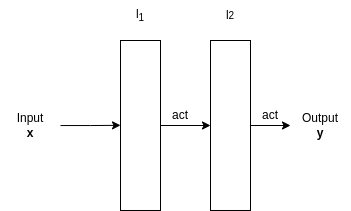
\includegraphics[width=0.5\textwidth]{../assets/nn-simple-example.png}
    \end{figure}
\end{frame}

\subsection{Fully connected layer}

\begin{frame}
    \frametitle{Fully connected layer}

    \begin{itemize}
        \item Used with convolutional layers
        \item Linearly seperable
    \end{itemize}

    \begin{columns}
        \begin{column}{0.5\textwidth}
            Example
            \begin{figure}
                \centering
                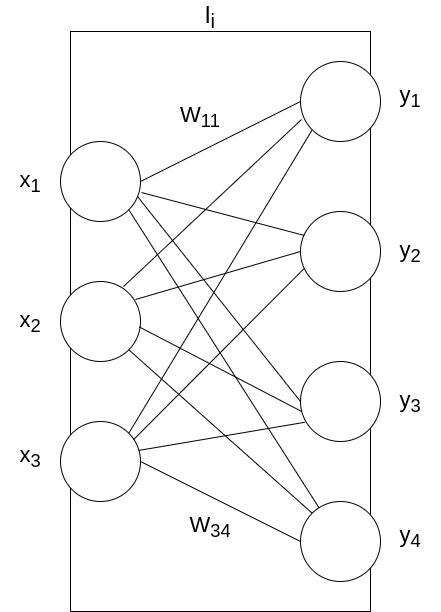
\includegraphics[width=0.6\textwidth]{../assets/linear-layer-example.png}
            \end{figure}
        \end{column}
        \pause
        \begin{column}{0.5\textwidth}
            General
            \begin{figure}
                \centering
                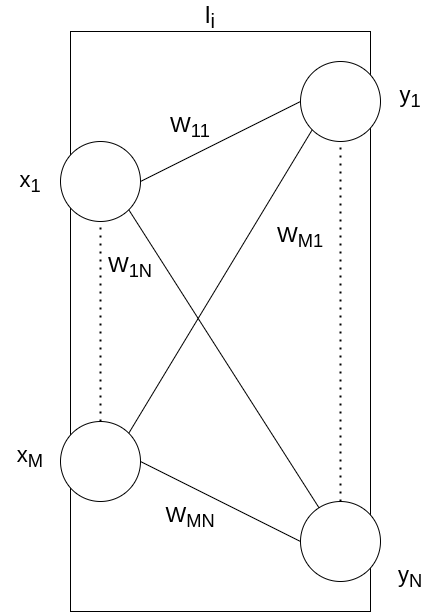
\includegraphics[width=0.6\textwidth]{../assets/linear-layer.png}
            \end{figure}
        \end{column}
    \end{columns}
\end{frame}

\begin{frame}
    \frametitle{Fully connected layer forward propagation}
    The value from each input $x_i$ is multiplied with a weight $w_{ij}$ and summed together in output $y_j$.
    \begin{itemize}
        \item Bias
    \end{itemize}

    \begin{figure}
        \centering
        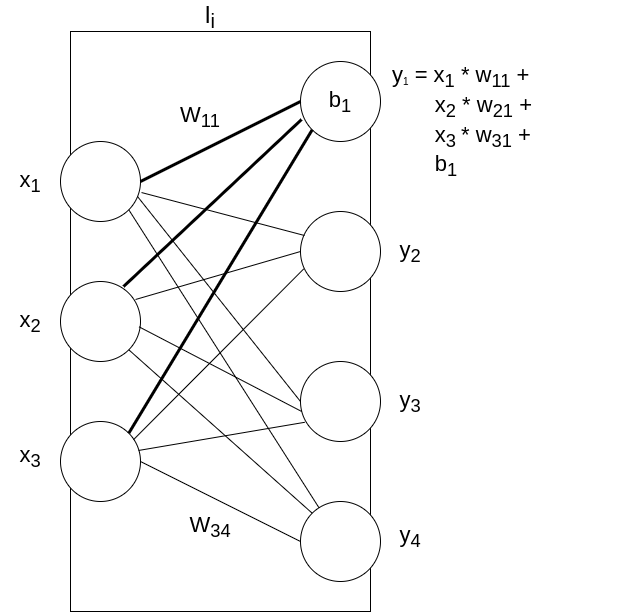
\includegraphics[width=0.5\textwidth]{../assets/linear-layer-linear-propagation.drawio.png}
    \end{figure}
\end{frame}

\begin{frame}
    \frametitle{Fully connected layer forward propagation}

    The forward propagation can be expressed as the following
    $$y_j = b_j + \sum^M_{i=1} w_{ji}x_i$$
    Where $j = 1...M$

    \pause
    And as an expression for all outputs
    $$\bm{y} = \bm{b} + \bm{Wx}$$
\end{frame}

\subsection{Activation functions}

\begin{frame}
    \frametitle{Activation Functions}
    Activation functions are applied to each value after a layer
    \begin{itemize}
        \item Non-linearity
        \item Better fitting
    \end{itemize}
    \pause

    \begin{table}[H]
    \centering
    \begin{tabular}{|c|c|}\hline
    \textbf{Function} & $\bm{\sigma}$ \\\hline
    tanh     & $\frac{e^x - e^{-y}}{e^x + e^{-y}}$ \\\hline
    ReLU     & $max(0, y)$ \\\hline
    sigmoid  & $\frac{1}{1+e^{-y}}$ \\\hline
    softmax  & $\frac{e^{y'}}{\sum^K_{k=1} e^{y_k}}$ \\\hline
    \end{tabular}
    \caption{A list of common activation functions.}
    \label{tab:activation}
    \end{table}
\end{frame}

\subsection{Convolutional layer}

\begin{frame}
    \frametitle{Convolutional layer}
    The convolutional layer is used to extract features from a structured data such as images.
    \begin{itemize}
        \item More layers $\rightarrow$ more features
    \end{itemize}
\end{frame}

\begin{frame}
    \frametitle{Convolutional layer}
    \begin{itemize}
        \item Input
        \item Channels
        \item Kernel
        \item Feature maps
    \end{itemize}
    \pause
    Consider the following input data and kernel

    \begin{figure}
        \centering
        \hfill
        \subfloat[][An example for a $3 \times 3$ input to a convolutional layer]{$\begin{bmatrix}
            X_{11} & X_{12} & X_{13} \\
            X_{21} & X_{22} & X_{23} \\
            X_{31} & X_{32} & X_{33} 
        \end{bmatrix}$}
        \hfill
        \subfloat[][An example for a $2\times 2$ kernel]{$\begin{bmatrix}
            K_{11} & K_{12} \\
            K_{21} & K_{22}
        \end{bmatrix}$}
        \hfill
        \null
        \caption{An example for an input and a kernel to be used in a convolutional layer}
        \label{fig:conv_input_and_kernel}
    \end{figure}
\end{frame}

\begin{frame}
    \frametitle{Convolutional layer example}

    \begin{figure}
        \centering
        $$\begin{bmatrix}
            \color{red} X_{11} & \color{red} X_{12} & X_{13} \\
            \color{red} X_{21} & \color{red} X_{22} & X_{23} \\
            X_{31} & X_{32} & X_{33} 
        \end{bmatrix} \otimes K \Rightarrow \begin{bmatrix}
            \color{red} X_{11} K_{11} + X_{12} K_{12} + X_{21} K_{21} + X_{22} K_{22} & \\
             &
        \end{bmatrix}$$\\
        \pause
        $$\begin{bmatrix}
            X_{11} & \color{red} X_{12} & \color{red} X_{13} \\
            X_{21} & \color{red} X_{22} & \color{red} X_{23} \\
            X_{31} & X_{32} & X_{33} 
        \end{bmatrix} \otimes K \Rightarrow \begin{bmatrix}
             Y''_{11} &\color{red} X_{12} K_{12} + X_{13} K_{13} + X_{22} K_{22} + X_{23} K_{23} \\
             &
        \end{bmatrix}$$\\
        \pause
        $$\begin{bmatrix}
            X_{11} & X_{12} & X_{13} \\
            \color{red} X_{21} & \color{red} X_{22} & X_{23} \\
            \color{red} X_{31} & \color{red} X_{32} & X_{33}
        \end{bmatrix} \otimes K \Rightarrow \begin{bmatrix}
            Y''_{11} & Y''_{12} \\
            \color{red} X_{21} K_{21} + X_{22} K_{22} + X_{31} K_{31} + X_{32} K_{32} & 
        \end{bmatrix}$$\\
        \pause
        $$\begin{bmatrix}
            X_{11} & X_{12} & X_{13} \\
            X_{21} & \color{red} X_{22} & \color{red} X_{23} \\
            X_{31} & \color{red} X_{32} & \color{red} X_{33}
        \end{bmatrix} \otimes K \Rightarrow \begin{bmatrix}
             Y''_{11} & Y''_{12} \\
             Y''_{21} & \color{red} X_{22} K_{22} + X_{23} K_{23} + X_{32} K_{32} + X_{33} K_{33}
        \end{bmatrix}$$\\
        \label{fig:conv_operation}
    \end{figure}
\end{frame}

\begin{frame}
    \frametitle{Convolutional layer stride example}
    A stride can also be used to reduce number of operations and downsample.

    \begin{figure}
        \centering
        $$\begin{bmatrix}
            \color{red} X_{11} & \color{red} X_{12} & X_{13} & X_{14} \\
            \color{red} X_{21} & \color{red} X_{22} & X_{23} & X_{24} \\
            X_{31} & X_{32} & X_{33} & X_{34}
        \end{bmatrix} \otimes K \Rightarrow ...$$\\
        $$\begin{bmatrix}
            X_{11} & X_{12} & \color{red} X_{13} & \color{red} X_{14} \\
            X_{21} & X_{22} & \color{red} X_{23} & \color{red} X_{24} \\
            X_{31} & X_{32} & X_{33} & X_{34}
        \end{bmatrix} \otimes K \Rightarrow ...$$\\
        \label{fig:conv_operation_with_stride}
    \end{figure}
\end{frame}

\begin{frame}
    \frametitle{Convolutional layer generalized}
    The outputs can be described as the following expression
    $$Y_{ij} = b + \sum^{C_{in}}_{c = 1} \sum^{i \cdot s_x + k_x}_{i_2 = i \cdot s_x} \sum^{j \cdot s_y + k_y}_{j_2 = j \cdot s_y} X_{ci_2j_2} K_{ci_2j_2} $$
    \pause

    \begin{description}
        \item[$C_{in}$] The number of in channels
        \item[$s_x$ $s_y$] The stride for each dimension
        \item[$k_x$ $k_y$] The size of the kernel
    \end{description}
    \pause

    $$i = 1, ..., \left\lfloor\frac{n_x - k_x}{s_x}\right\rfloor + 1$$
    $$j = 1, ..., \left\lfloor\frac{n_y - k_y}{s_y}\right\rfloor + 1$$

    \begin{description}
        \item[$n_x$ $n_y$] The size of the input
    \end{description}
\end{frame}

\subsection{Maxpooling layer}

\begin{frame}
    \frametitle{Maxpooling layer}

    \begin{itemize}
        \item Downsampling to avoid overfitting
        \item Feature maps
        \pause
        \item Partitioning $\rightarrow$ max
    \end{itemize}


    \begin{figure}[htpb]
        \centering
        $$\begin{bmatrix}
            \color{red}1 & \color{red} 2 & \color{green} 3 & \color{green} 4 \\
            \color{red}8 & \color{red}9 & \color{green}10 & \color{green}11 \\
            \color{blue}7 & \color{blue}1 & \color{magenta}2 & \color{magenta}6 \\
            \color{blue}2 & \color{blue}1 & \color{magenta}9 & \color{magenta}3
            \end{bmatrix} \Rightarrow \begin{bmatrix}
            \color{red}9 & \color{green}11 \\
            \color{blue}7 & \color{magenta}9
            \end{bmatrix}$$
        \caption{Illustration of a max pooling operation on a $4\times 4$ matrix with a $2\times 2$ window. The window will process the numbers of the same color and output the same color.}
        \label{fig:max_pool}
    \end{figure}
\end{frame}

\subsection{Loss functions}

\begin{frame}
    \frametitle{Loss functions}

    \begin{itemize}
        \item How close at predicting
        \item important for training
    \end{itemize}

    \begin{table}[ht]
        \centering
        \begin{tabular}{|c|c|}
        \hline
        \textbf{Loss function}  & $L\bm{(y, l)$} \\ \hline
        Cross entropy  & $-\sum^K_{k=1}(l_k\ ln\ y_k)$ \\ \hline
        Mean squared error & $\frac{1}{K}\sum^K_{k=1}(y_k-l_k)^2$ \\ \hline
        \end{tabular}
        \caption{Some common loss functions, where $\bm{y}$ is the output of the network and $\bm{l}$ is the expected values or labels}
        \label{tab:loss}
    \end{table}
\end{frame}

\subsection{Network training}

\begin{frame}
    \frametitle{Network training}

    \begin{itemize}
        \item Fitting the network to some data
        \item Predicting
    \end{itemize}

    \pause

    The network can be trained with the help of a loss function and gradient descent

    \pause

    Consider the loss function of a network
    $$L(f(\bm{x}, \bm{W}), \bm{l})$$
    Note $f$ is the forward propagation function of the network,
    \pause
    while $\bm{l}$ is the labels.

    \pause
    Since the loss will not get below zero, we can attempt to find a minima of the loss function.
\end{frame}

\begin{frame}
    \frametitle{Network training}

    By using gradient descent, we might find a minima of the loss function.
    \pause
    First we find the gradient with respect to $\bm{W}$.
    $$\nabla_{\bm{W}} L(f(\bm{x}, \bm{W}), \bm{l})$$
    \pause
    By using gradient descent and always updating $\bm{W}$, we might find some optimal values for $\bm{W}$.
    \pause

    We initialize $\bm{W}_0$ to some random weights. Then
    \pause
    $$\bm{W}_1 \leftarrow \bm{W}_0 - \nabla_{\bm{W}}L(f(\bm{x}, \bm{W}_0), \bm{l})$$
    \pause
    $$\bm{W}_2 \leftarrow \bm{W}_0 - \nabla_{\bm{W}}L(f(\bm{x}, \bm{W}_1), \bm{l})$$
    ...
\end{frame}

\subsection{Exploding/vanishing gradients}

\subsection{Barch normalization layer}

\subsection{ResNet}

\begin{frame}
    \frametitle{ResNet}
\end{frame}

\section{Automatic differentiation}

\subsection{Methods of differentitation}

\subsection{Automatic differentitaion}

\subsection{Forward mode}

\subsection{Reverse mode}

\section{Optimizing matrix multiplication}

\section{Design and implementation}

\section{Future work and conclusion}

\section{Benchmarking}

\begin{frame}
    \begin{itemize}
        \item Attempted to benchmark with the MNIST numbers dataset
    \end{itemize}
\end{frame}

\subsection{Future work}

\subsection{Conclusion}

\end{document}
